%%%%%%%%%%%%%%%%%%%%%%%%%%%%%%%%%%%%%%%%%%%%%%
\logvartrue
\chapter{Small tools for big data}
%%%%%%%%%%%%%%%%%%%%%%%%%%%%%%%%%%%%%%%%%%%%%%
Working with metagenomic data involves the need to handle huge amounts of data obtained from different conditions and environments. Dealing with these ``big data'' is a non-trivial task both from a biological and computation point of view. Indeed, the collection and storage of metagenomic data requires significant infrastructure and have greatly benefited from the use of cloud computing. The global information storage capacity has almost doubled every four years since the 1980s, collecting larger and larger data sets both from genomic and metagenomic projects. New databases (like SRA) make raw DNA sequences and other primary data available to researchers and represent new insights waiting to be found. However, what are needed now are robust analysis tools able to mine the data to find new insights among members of bacterial communities, informing on their chemistry and biology. For this reason ``big data'' analytic tools will be an invaluable resource for deeply understanding microbiome data in order to develop new solutions to global health problems and provide new insights into microbiology.\\


\section{Raw Sequence Data and Quality Control}
As said, the use of next-generation sequencing technologies has increased over the past decade. One of the problems, related to the utilization of this kind of data, is the pre-processing of raw sequences produced by sequencing machines. This step involves: sequence improvement, removal (trimming) of low-quality segments and deletion of contaminants. Here, is reported a series of useful methods for dealing with metagenomic (and genomic) data. One of the methods proposed, based on dynamic trimming, as implemented in the software StreamingTrim allows a fast and accurate trimming of sequence files, with low memory requirement.\\
\newpage
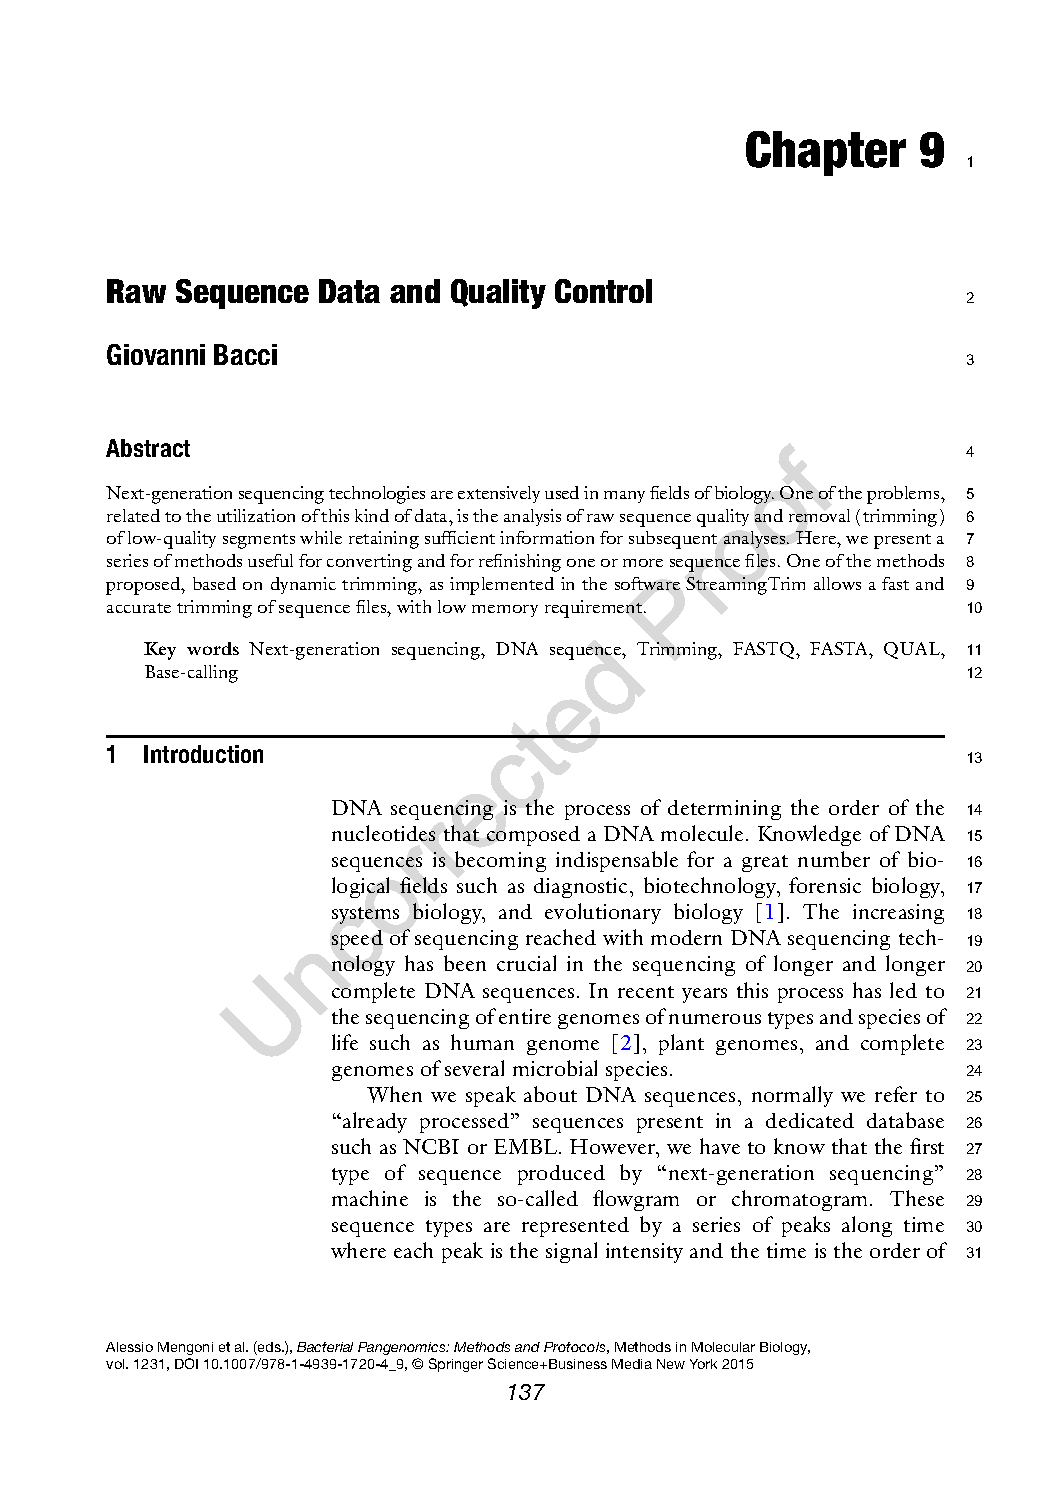
\includepdf[pages=-,offset=10mm 0, scale=0.9]{articles/book.pdf}
\newpage

\section{Evaluation of the performances of Ribosomal Database Project (RDP) Classifier for taxonomic assignment of 16S rRNA metabarcoding sequences generated from Illumina-Solexa NGS}
Here we report a benchmark of the effect of bootstrap cut-off values of the RDP Classifier tool in terms of data retention along the different taxonomic ranks by using Illumina reads. Results provide guidelines for planning sequencing depths and selection of bootstrap cut-off in taxonomic assignments.\\

\subsection{Introduction}
The use of 16S rRNA massive sequencing has deeply improved the technical possibilities to describe the taxonomic composition and functionality of microbial communities \cite{degnan2011illumina}. Following the reduction in DNA sequencing cost, many studies have been performed using amplicon libraries to taxonomically describe microbial communities in many different environments. The large number of sequence reads can be taxonomically assigned by comparison with taxonomically classified sequences present in dedicated databases of 16S rRNA genes, as for instance SILVA \cite{quast2012silva}, Greengenes \cite{desantis2006greengenes} or the Ribosomal Database Project \cite{wang2007naive}. In particular, one of the most popular tool used to assign sequence reads to the prokaryotic taxonomy is the Na\"ive Bayesian Classifier tool hosted by Ribosomal Database Project (RDP Classifier) \cite{wang2007naive}. The RDP Classifier tool uses a very fast algorithm, based on the Bayes' theorem, suitable for the analysis of large amount of sequence data. This algorithm has been tested on near-full-length 16S rRNA sequences and on randomly generated 16S rRNA sequence fragments of 400, 200, 100 and 50 bases in length from a number (5,014) of type strains belonging to 988 genera \cite{wang2007naive}. An overall accuracy of above 88.7\% and 83.2\% for 400 and 200 base segments, respectively (very similar to the accuracy obtained with the near-full-length 16S rRNA sequence) was reported \cite{wang2007naive}. Moreover, an average accuracy at genus level of 71.1\% and 51.5\% for the 100 and the 50 base segments respectively was found. However, these results have been obtained using a 16S rRNA sequence fragments dataset built with sequences derived from well taxonomically defined organisms. No data have been reported on datasets composed by 16SrRNA sequences from particular regions of the 16S molecule (e.g. V3 and V6) and obtained after amplification of DNA from environmental samples. \\
In the last years, Illumina sequencing technology has emerged as one of the most popular sequencing technology, thanks to the lower prices, higher number of generated sequences and accuracy than pyrosequencing and Ion Torrent technologies \cite{degnan2011illumina, gloor2010microbiome, bartram2011generation, claesson2010comparison, salipante2014performance}. In particular, different Illumina platforms are available (with different cost of sequencing) which provide different number of reads and different reads lengths (see for instance \href{http://www.illumina.com/systems/sequencing.ilmn}{http://\-www.\-illumi\-na\-.com/\-sys\-tems/\-sequen\-cing\-.ilmn}). Additionally, Illumina reads are usually 100-200 nt long (depending on the techniques used) and 16S rRNA amplicon studies have focused on single variable regions of the 16S rRNA gene, as the V3, V4 or V6, which are approximately 100-300 bp long. Consequently, a concern about the amount of reads to generate and the setting of the bootstrap threshold of RDP Classifier to provide biologically meaningful data is present. More specifically, there is a lack of information on the percentage of reads which can be assigned to the various phylogenetic levels with Illumina 16S rRNA metabarcoding.\\

\subsection{Results and Discussion}
Here, we report a benchmark of RDP Classifier based on environmental sequence datasets obtained with Illumina sequencing technology. In particular, we investigated the effect of bootstrap cutoff values on the accuracy of taxonomic attribution of Illumina reads. Results obtained provide a guideline for the selection of optimal bootstrap cutoff values in terms of data retention along the different taxonomic ranks.\\
\begin{table}
\centering
\scriptsize
\begin{tabular}{ p{0.12\textwidth} p{0.06\textwidth} p{0.06\textwidth} p{0.06\textwidth} p{0.08\textwidth} p{0.4\textwidth} }
\hline
BioProject & Region & Length & Samples & Sequences & Environment\\
\hline\hline
PRJEB6047 & V3 & 302bp & 72 & 61023 & Subgingival, supragingival, and tongue plaque from healthy and periodontal subjects \\
PRJNA245381 & V3 & 300bp & 100 & 28634 & Soil contaminated with increasing level of ionic Ag\\
PRJNA217938 & V4 & 288bp & 25 & 476230 & Samples from the surface to depth in Upper Mystic Lake, Winchester, MA\\
PRJNA238275 & V4 & 251bp & 6 & 759518 & Soil associated with the rhizosphere of the coffee plant (\textit{Coffea canephora}) in Brazil\\
PRJNA188383 & V6 & 200bp & 48 & 66887 & Seawater and surface sediments retrieved from the Arctic Ocean\\\hline 
\end{tabular}
\caption{\label{tab:1rdp}Description of the datasets used. ``BioProject'' = accession ID (\href{http://www.ncbi.nlm.nih.gov/bioproject/}{http://\-www.\-ncbi.\-nlm.\-nih\-.gov/\-biopro\-ject/}); ``Region'' = rRNA gene variable region; ``Lenght'' = average read length; ``Samples'' = number of samples; ``Sequences'' = average number of sequences per sample; ``Environment'' = the environment where the study has been conducted.}
\end{table}
Five datasets of 16S rRNA gene Illumina reads, generated from environmental DNA, were analyzed (Table~\ref{tab:1rdp}). These datasets contains a high number of reads per sample (from 28,634 to 759,518 reads per sample) and are including reads obtained from V3, V4 and V6 regions.. Reads present in the analyzed datasets were trimmed with StreamingTrim version 1.0 [9], before taxonomic assignment with the RDP Classifier. The proportion of assigned reads in relation to the bootstrap cutoff value (from 0.1 to 1.0 with an increment of 0.1) for each taxonomic level (from \textit{domain} to \textit{genus}) is reported in Figure~\ref{tab:1rdp}. As expected, the proportion of assigned reads decreased going down along taxonomic levels from \textit{phylum} (from a mean of 100\% to a mean of 25\%, in the two datasets) to \textit{genus} (from a mean of 60\% to a mean of smaller than 5\%, in the two datasets). In particular it is worth noticing that all datasets, which included three variable regions (V3, V4 and V6) of 16S rRNA gene, more than 25\% of the reads could be assigned to the family level using a bootstrap cutoff value of 0.5 (the default cut-off value reported in the RDP Classifier tutorial). Moreover, even at higher cutoff values ({\textgreater} 0.8) an appreciable number of reads were still assigned (5\% - 10\%). Interestingly, the V3 region performed better in the taxonomic attribution at Order and Family levels, indicating that even highly stringent bootstrap cut-off values (e.g. 0.7) may allow to assign more reads from V3 region than from V4 and V6 region, which consequently resulted less taxonomically informative.\\
\begin{figure}[!tb]
	\centering
	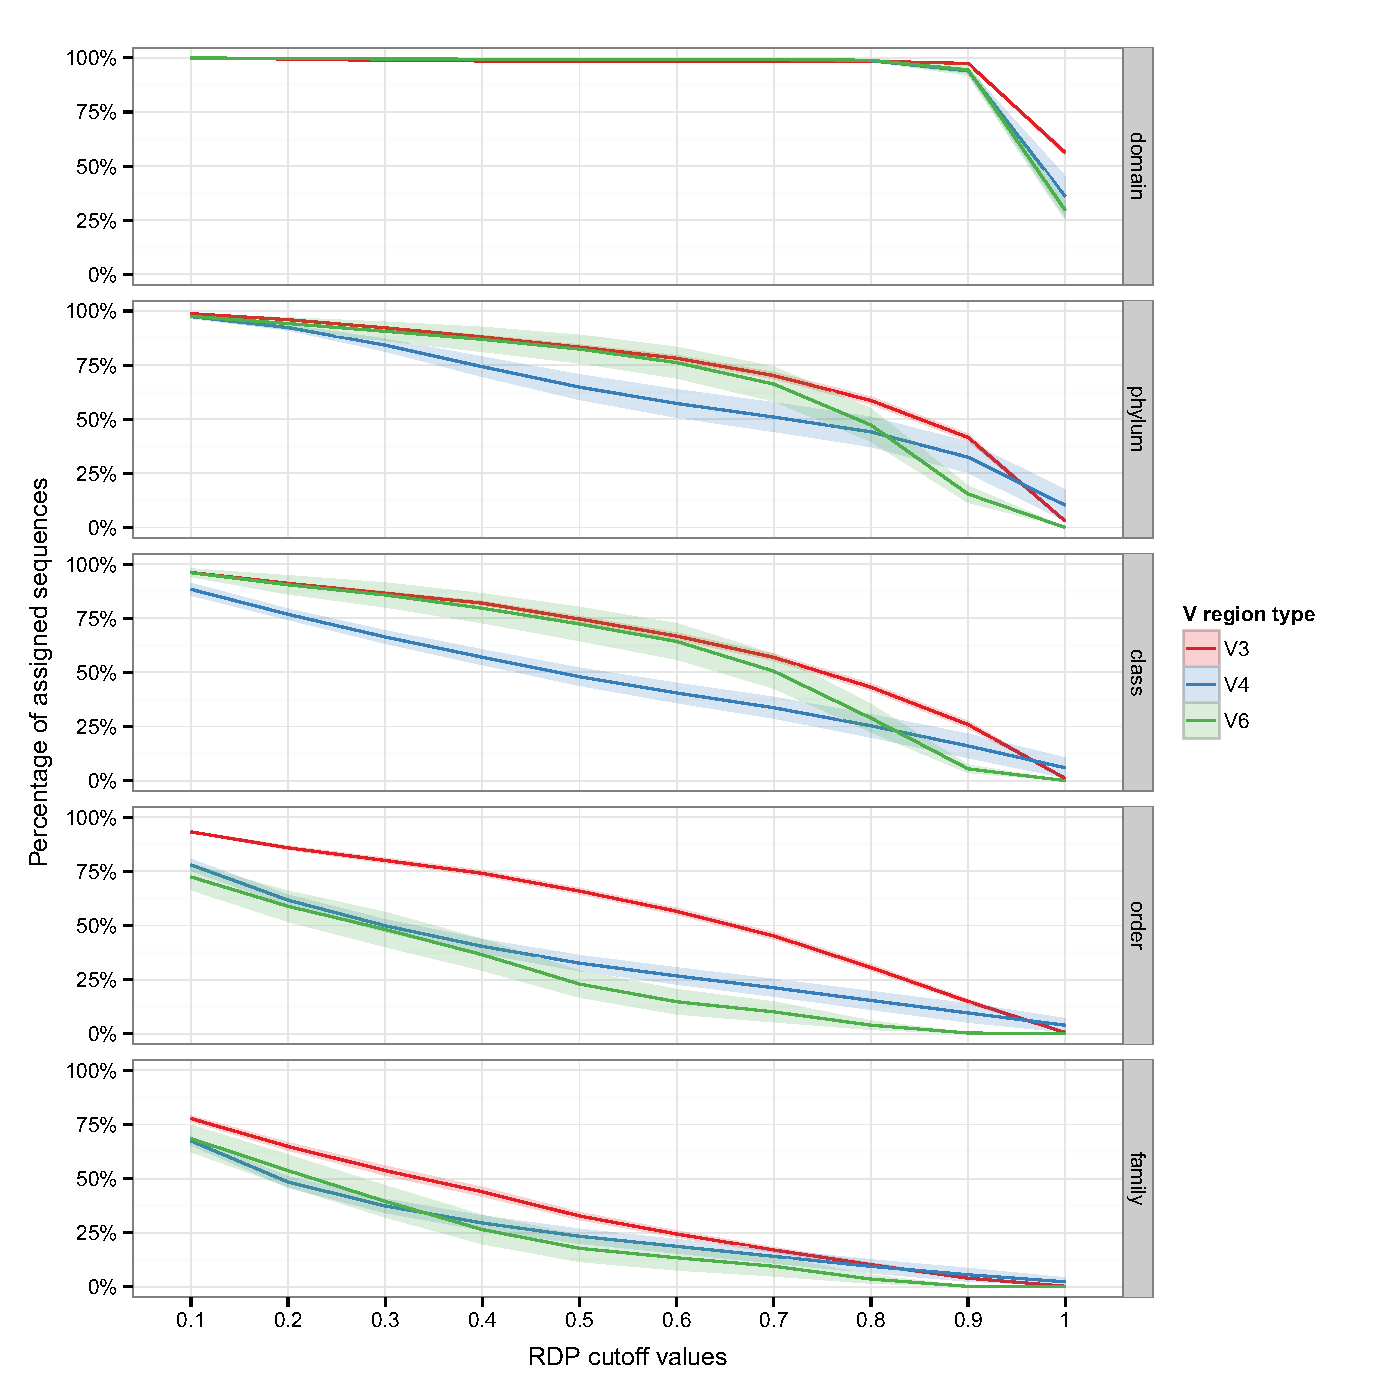
\includegraphics[width=0.8\textwidth]{./figures/Chapter_2/Figure_1}
  	\caption{\label{fig:1rdp}Effect of bootstrap cut-off thresholds on the number of reads. The percentage of trimmed reads assigned to each taxonomic level is reported versus RDP bootstrap cut-off values. Shaded lines correspond to the 95\% confidence interval assuming normality.}
\end{figure}
The assignments trend at the \textit{genus} level (the lower taxonomic level that can be obtained using the RDP Classifier) was then inspected (Figure~\ref{fig:2rdp}).  Here also, V3 region better performed than V4 and V6 region in the retention of taxonomic information lowering bootstrap values, especially at bootstrap cutoff value of 0.5 and lower. A pseudo-fit of curve was also produced (Supplemental Figure SM1), which may allow researchers to infer the percentage of sequences that could be assigned to the \textit{genus} level at different RDP bootstrap cut-offs.\\
\begin{figure}[!tb]
	\centering
	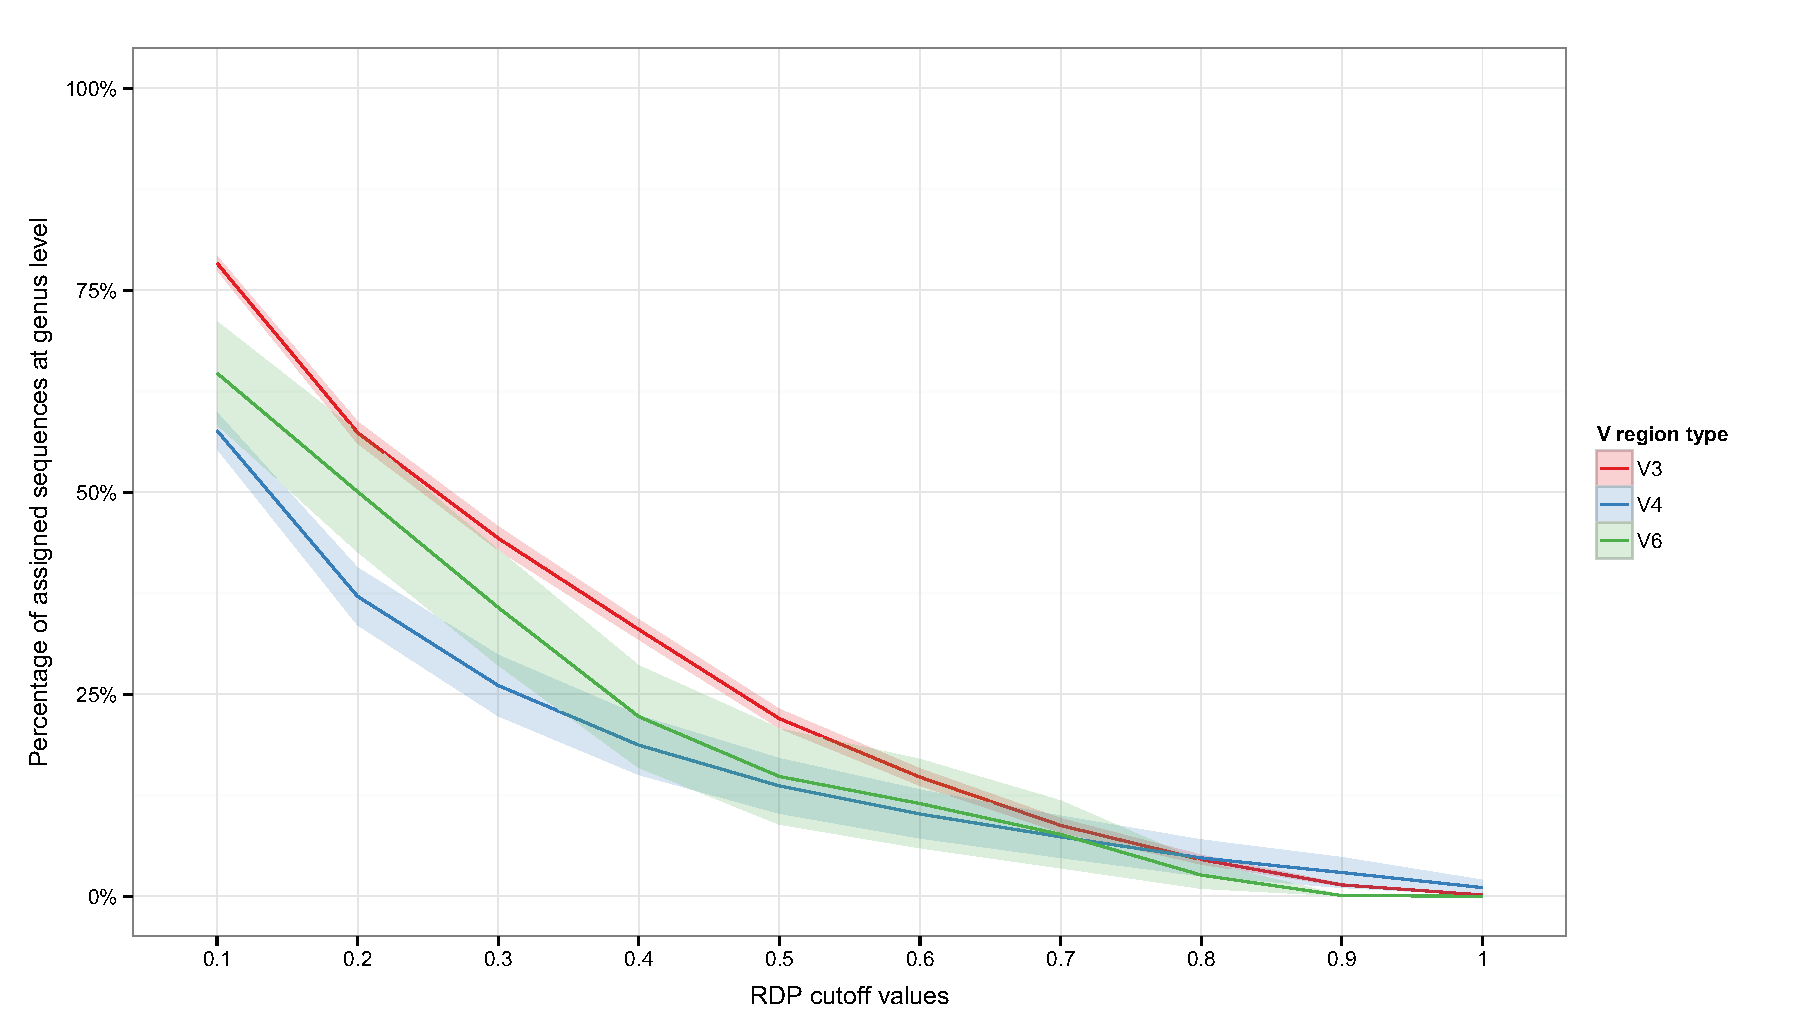
\includegraphics[width=0.8\textwidth]{./figures/Chapter_2/Figure_2}
  	\caption{\label{fig:2rdp}Percentage of assigned reads with respect to bootstrap cut-off thresholds at the genus level. Plots report the assigned reads for all dataset analyzed. Shaded lines correspond to the 95\% confidence interval assuming normality.}
\end{figure}
In conclusion, Illumina reads, shorter than 200 nt, can be classified using one of the most common 16S rRNA sequence classifier: the RDP Classifier. As one would expect, the increase of the bootstrap cutoff value leads to a decreased number of assigned sequences. However, even at cutoffs higher than those indicated in the RDP Classifier tutorial, approximately 20-30\% of the analyzed reads were still assigned. These results indicate that Illumina-based metabarcode sequencing of 16S rRNA gene can provide reliable information for taxonomic composition of a community at the genus level even using classification software not specifically designed for this type of sequences. The reported models for trend plots can guide experimentalists in choosing the sequencing depth more adapted for retaining an appreciable number of assigned reads different taxonomic resolution.\\

\subsection{Acknowledgments}
This work was supported by a grant from the Ente Cassa di Risparmio di Firenze (Grant n{\textdegree} 2010/4384 ``Centro di Metagenomica del suolo'') and by a fellowship to GB from MIPAAF.

\section{StreamingTrim 1.0: a Java software for dynamic trimming of 16S rRNA sequence data from metagenetic studies}
The so-called barcode or metagenetic applications, based on PCR amplicon library sequencing, are very popular at present. One big problem, related to the utilization of amplicon data, is the analysis of reads quality and the removal of low-quality regions without deleting entire sequences which can be useful for subsequent analyses (e.g. taxonomic assignment). Here, we present StreamingTrim, a DNA reads trimming software, written in Java, that allows researchers to analyse the quality of DNA sequences in fastq files searching and removing low-quality regions in a very conservative way.\\
\newpage
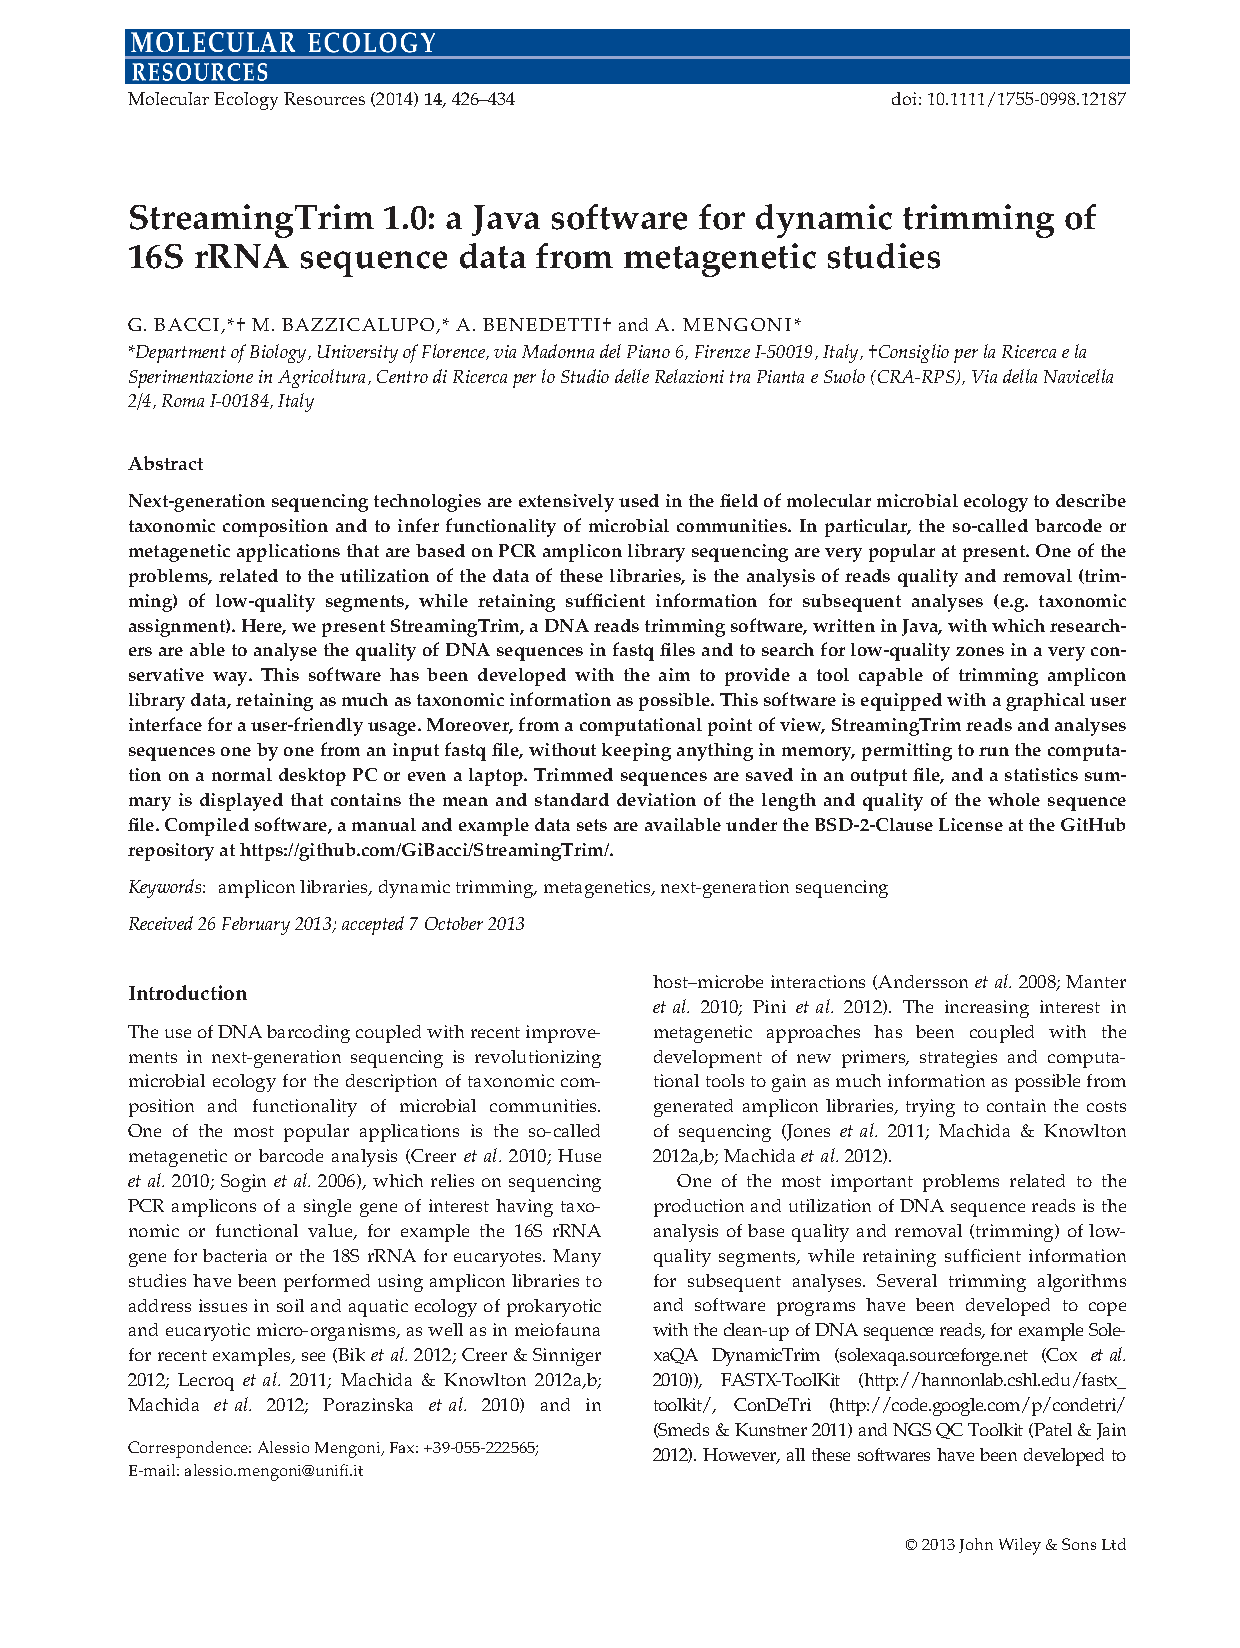
\includepdf[pages=-,offset=10mm 0, scale=0.9]{articles/StremingTrim.pdf}
\newpage

%%-----------
%% Backmatter
%%-----------
\backmatter
\chaptermark{Bibliography}
\renewcommand{\sectionmark}[1]{\markright{#1}}
\bibliographystyle{unsrt}                           %Use alpha codes for references
\sectionmark{Bibliography}
\addcontentsline{toc}{chapter}{Bibliography}        %Force addition of Bibliography to TOC    
\bibliography{References}